\mxfront{stmg-bank-b}

% -----------------------------------------------------------------------------
% Chapitre 3 -- Fonction logarithme décimal
% -----------------------------------------------------------------------------
\mxexdef{15}{Isoler $10^x$ puis passer au logarithme}{%
Résoudre dans $\R$ les équations suivantes. Lorsqu'une solution existe, donner sa valeur exacte puis sa valeur arrondie au millième.
\begin{enumerate}[label=\alph*.]
\item $4\times10^x=9{,}2$
\item $7\times10^x-1{,}5=3\times10^x+0{,}9$
\item $2{,}5\times10^x+12=6-0{,}5\times10^x$
\item $10^{x+1}=50$ \quad (on pourra écrire $10^{x+1}=10\times10^x$)
\end{enumerate}
}{%
Méthode : regrouper les termes en $10^x$ d'un côté, isoler $10^x$, vérifier que le second membre est strictement positif, puis utiliser : pour $b>0$, $10^x=b \iff x=\log(b)$.
\begin{enumerate}[label=\alph*.]
\item $10^x=\dfrac{9{,}2}{4}=2{,}3>0$, donc $x=\log(2{,}3)\approx0{,}362$.
\item $7\times10^x-3\times10^x=0{,}9+1{,}5$, soit $4\times10^x=2{,}4$, donc $10^x=0{,}6>0$ et $x=\log(0{,}6)\approx-0{,}222$.
\item $2{,}5\times10^x+0{,}5\times10^x=6-12$, soit $3\times10^x=-6$, donc $10^x=-2$. Or $10^x>0$ pour tout réel $x$ : l'équation n'a aucune solution.
\item $10\times10^x=50$, donc $10^x=5>0$ et $x=\log(5)\approx0{,}699$. (Autre écriture : $x+1=\log(50)$, donc $x=\log(50)-1=\log(5)$.)
\end{enumerate}
Contrôle conseillé à la calculatrice : $10^{0{,}362}\approx2{,}30$ et $10^{-0{,}222}\approx0{,}60$.
}{4}

\mxexdef{16}{Signe d'un logarithme et comparaison}{%
On rappelle que la fonction $\log$ est strictement croissante sur $]0;+\infty[$ et que $\log(1)=0$.
\begin{enumerate}
\item Sans calculatrice, donner le signe de chacun des nombres suivants, en justifiant :
\begin{enumerate}[label=\alph*.]
\item $\log(0{,}9)$ ;
\item $\log\!\left(\dfrac{4}{3}\right)$ ;
\item $\log(CM)$, où $CM$ est le coefficient multiplicateur associé à une hausse de $0{,}2\,\%$.
\end{enumerate}
\item Sans calculatrice, comparer $\log(0{,}35)$ et $\log(0{,}53)$.
\end{enumerate}
}{%
\begin{enumerate}
\item Pour $a>0$ : si $a>1$ alors $\log(a)>\log(1)=0$ ; si $0<a<1$ alors $\log(a)<0$ (croissance stricte de $\log$).
\begin{enumerate}[label=\alph*.]
\item $0<0{,}9<1$, donc $\log(0{,}9)<0$ (environ $-0{,}046$).
\item $\dfrac43>1$, donc $\log\!\left(\dfrac43\right)>0$ (environ $0{,}125$).
\item $CM=1+\dfrac{0{,}2}{100}=1{,}002>1$, donc $\log(1{,}002)>0$ (environ $0{,}000\,87$, très proche de $0$ mais positif).
\end{enumerate}
\item $0<0{,}35<0{,}53$ et $\log$ est strictement croissante sur $]0;+\infty[$, donc $\log(0{,}35)<\log(0{,}53)$. Les deux nombres sont négatifs (arguments inférieurs à $1$) ; le plus proche de $0$ est $\log(0{,}53)$.
\end{enumerate}
}{3}

\mxexdef{17}{Condenser une expression en un seul logarithme}{%
Écrire chacun des nombres suivants sous la forme $\log(A)$, où $A$ est un nombre réel strictement positif à préciser sous forme entière ou fractionnaire. Lorsque c'est possible, donner la valeur exacte du nombre.
\begin{enumerate}[label=\alph*.]
\item $\log(6)+\log(5)-\log(3)$
\item $2\log(4)-\log(8)$
\item $\log(5)+\log(11)$
\item $2\log(3)-3\log(2)$
\item $\log(40)-\log(8)+2\log(2)$
\end{enumerate}
}{%
On utilise, pour $a,b>0$ et $n$ entier naturel : $\log(a)+\log(b)=\log(ab)$, $\log(a)-\log(b)=\log\!\left(\dfrac ab\right)$ et $n\log(a)=\log(a^n)$. Tous les arguments sont strictement positifs.
\begin{enumerate}[label=\alph*.]
\item $\log(6)+\log(5)-\log(3)=\log\!\left(\dfrac{6\times5}{3}\right)=\log(10)=1$.
\item $2\log(4)-\log(8)=\log(4^2)-\log(8)=\log\!\left(\dfrac{16}{8}\right)=\log(2)$.
\item $\log(5)+\log(11)=\log(55)$.
\item $2\log(3)-3\log(2)=\log(3^2)-\log(2^3)=\log\!\left(\dfrac98\right)$.
\item $\log(40)-\log(8)+2\log(2)=\log\!\left(\dfrac{40\times2^2}{8}\right)=\log(20)$.
\end{enumerate}
Erreur à signaler : $\log(5)+\log(11)$ n'est pas $\log(16)$ ; une somme de logarithmes correspond à un produit des arguments.
}{4}

\mxexdef{18}{Algorithme de seuil pour une évolution}{%
Une entreprise de livraison achète une camionnette $38\,000$~€. On estime que sa valeur diminue de $15\,\%$ chaque année. L'entreprise revendra la camionnette dès que sa valeur deviendra strictement inférieure à $10\,000$~€.
On note $V$ la valeur de la camionnette (en euros) et $N$ le nombre d'années écoulées depuis l'achat.
\begin{center}
\begin{tabular}{|l|}
\hline
$V\leftarrow38\,000$\\
$N\leftarrow0$\\
Tant que $V\ \ldots\ldots\ldots$\\
\hspace*{1.5em}$V\leftarrow\ldots\ldots\ldots$\\
\hspace*{1.5em}$N\leftarrow N+1$\\
Fin Tant que\\
\hline
\end{tabular}
\end{center}
\begin{enumerate}
\item Compléter l'algorithme pour qu'à la fin de son exécution, la variable $N$ contienne le nombre d'années au bout duquel la camionnette sera revendue.
\item À l'aide de la calculatrice (tableau de valeurs), faire tourner l'algorithme et déterminer la valeur de $N$ obtenue. Donner la valeur de la camionnette au moment de la revente, arrondie à l'euro.
\item Écrire ce programme en langage Python, l'exécuter et comparer avec le résultat de la question 2.
\end{enumerate}
}{%
\begin{enumerate}
\item Une baisse de $15\,\%$ correspond au coefficient multiplicateur $1-0{,}15=0{,}85$. On répète tant que la valeur n'est pas encore passée sous le seuil : « Tant que $V\geqslant10\,000$ » et « $V\leftarrow0{,}85\times V$ ».
\item Valeurs successives arrondies à l'euro : $N=6$ : $14\,332$~€ ; $N=7$ : $12\,182$~€ ; $N=8$ : $10\,355$~€ ; $N=9$ : $8\,801$~€.
Comme $38\,000\times0{,}85^8\approx10\,355\geqslant10\,000$ et $38\,000\times0{,}85^9\approx8\,801<10\,000$, la boucle s'arrête avec $N=9$ : la camionnette sera revendue au bout de $9$ ans, pour une valeur d'environ $8\,801$~€.
\item Programme possible :\\
\texttt{V = 38000}\\
\texttt{N = 0}\\
\texttt{while V >= 10000:}\\
\hspace*{2em}\texttt{V = 0.85 * V}\\
\hspace*{2em}\texttt{N = N + 1}\\
\texttt{print(N, V)}\\
Le programme affiche $9$ et environ $8801{,}44$, ce qui confirme la question 2. Insister sur le point décimal en Python et sur l'indentation du bloc de la boucle.
\end{enumerate}
}{5}

\mxexdef{19}{Temps de doublement et dépassement}{%
Une boutique en ligne A a enregistré $2\,500$ commandes en janvier 2026. On suppose que ce nombre augmente de $7\,\%$ par mois. On note $a_n$ le nombre de commandes $n$ mois après janvier 2026.
\begin{enumerate}
\item
\begin{enumerate}[label=\alph*.]
\item Exprimer $a_n$ en fonction de $n$.
\item Au bout de combien de mois le nombre mensuel de commandes aura-t-il doublé ?
\item Au bout de combien de mois aura-t-il quadruplé ? Ce résultat est-il le double du précédent ? Expliquer.
\end{enumerate}
\item Une boutique concurrente B a enregistré $4\,000$ commandes en janvier 2026, avec une hausse de $3\,\%$ par mois. À partir de combien de mois la boutique A aura-t-elle plus de commandes mensuelles que la boutique B ? En quel mois cela se produira-t-il ?
\end{enumerate}
}{%
\begin{enumerate}
\item
\begin{enumerate}[label=\alph*.]
\item Une hausse de $7\,\%$ correspond au coefficient $1{,}07$ : $a_n=2\,500\times1{,}07^n$.
\item $a_n\geqslant5\,000\iff1{,}07^n\geqslant2\iff n\log(1{,}07)\geqslant\log(2)\iff n\geqslant\dfrac{\log(2)}{\log(1{,}07)}$, car $\log(1{,}07)>0$ (on ne change pas le sens de l'inégalité). Or $\dfrac{\log 2}{\log 1{,}07}\approx10{,}24$ : il faut $11$ mois. Contrôle : $1{,}07^{10}\approx1{,}967<2$ et $1{,}07^{11}\approx2{,}105\geqslant2$.
\item $1{,}07^n\geqslant4\iff n\geqslant\dfrac{\log(4)}{\log(1{,}07)}\approx20{,}49$ : il faut $21$ mois ($1{,}07^{20}\approx3{,}870$ et $1{,}07^{21}\approx4{,}141$). Comme $\log(4)=2\log(2)$, le seuil exact est bien le double ($20{,}49=2\times10{,}24$), mais l'arrondi à l'entier supérieur ne se fait qu'une fois : $21$ et non $2\times11=22$.
\end{enumerate}
\item On cherche $n$ tel que $2\,500\times1{,}07^n>4\,000\times1{,}03^n$. En divisant par $2\,500\times1{,}03^n>0$ : $\left(\dfrac{1{,}07}{1{,}03}\right)^n>1{,}6$. Comme $\dfrac{1{,}07}{1{,}03}>1$, son logarithme est positif et $n>\dfrac{\log(1{,}6)}{\log(1{,}07/1{,}03)}\approx12{,}34$. Il faut donc $n=13$ : contrôle $a_{12}\approx5\,630<5\,703$ et $a_{13}\approx6\,025>5\,874$. La boutique A dépassera B en février 2027 ($13$ mois après janvier 2026).
\end{enumerate}
}{5}

\mxexdef{20}{Trouver un taux : équation $x^n=b$}{%
Le prix public d'un modèle de panneau solaire est passé de $420$~€ en mars 2021 à $260$~€ en septembre 2025, soit une durée de $4$ ans et $6$ mois. On suppose que le prix a évolué à un taux annuel constant $t$.
\begin{enumerate}
\item Justifier que $(1+t)^{4{,}5}=\dfrac{260}{420}$.
\item En déduire $t$, arrondi à $0{,}1\,\%$. Interpréter le signe du résultat.
\item Un second modèle coûte aujourd'hui $395$~€. Si son prix évolue au même taux annuel, quel sera son prix dans $2$ ans et $3$ mois ? Arrondir à l'euro.
\item Le fabricant de ce second modèle souhaite plutôt atteindre un prix de $300$~€ dans $2$ ans et $3$ mois. Quel taux annuel constant doit-il appliquer ? Arrondir à $0{,}1\,\%$.
\end{enumerate}
}{%
\begin{enumerate}
\item Sur une durée de $4{,}5$ ans, le prix est multiplié par $(1+t)^{4{,}5}$, donc $420(1+t)^{4{,}5}=260$, soit $(1+t)^{4{,}5}=\dfrac{260}{420}\approx0{,}619$.
\item $1+t>0$, donc $1+t=\left(\dfrac{260}{420}\right)^{1/4{,}5}\approx0{,}8989$, d'où $t\approx-0{,}101$, soit $t\approx-10{,}1\,\%$. Le taux est négatif : le prix a baissé en moyenne d'environ $10{,}1\,\%$ par an. Contrôle : $420\times0{,}8989^{4{,}5}\approx260$.
\item $2$ ans et $3$ mois $=2{,}25$ ans. Prix : $395(1+t)^{2{,}25}$. En gardant la valeur exacte de $1+t$ en mémoire : $395\times\left(\dfrac{260}{420}\right)^{2{,}25/4{,}5}=395\times\left(\dfrac{260}{420}\right)^{0{,}5}\approx395\times0{,}7868\approx310{,}78$. Le prix serait d'environ $311$~€.
\item On résout $395(1+t')^{2{,}25}=300$, soit $(1+t')^{2{,}25}=\dfrac{300}{395}\approx0{,}7595$, donc $1+t'=\left(\dfrac{300}{395}\right)^{1/2{,}25}\approx0{,}8849$ et $t'\approx-11{,}5\,\%$. Il faudrait une baisse d'environ $11{,}5\,\%$ par an.
\end{enumerate}
Remarque : utiliser une valeur de $t$ arrondie trop tôt modifie légèrement les résultats (par exemple $395\times0{,}899^{2{,}25}\approx310{,}85$) ; garder la valeur en mémoire.
}{4}

\mxexdef{21}{Utiliser une formule $\log(N)/\log(2)$}{%
En laboratoire, une culture de cellules se multiplie par divisions successives : à chaque génération, le nombre de cellules double. Lorsque le nombre de cellules passe de $N_0$ à $N$, le nombre de générations écoulées est
\[
g=\frac{\log\!\left(\dfrac{N}{N_0}\right)}{\log(2)}.
\]
Par exemple, passer de $1$ à $8$ cellules correspond à $g=\dfrac{\log(8)}{\log(2)}=3$ générations.
\begin{enumerate}
\item Une culture passe de $1\,000$ à $64\,000$ cellules. Combien de générations se sont écoulées ?
\item Une autre culture passe de $500$ à $128\,000$ cellules. Même question.
\item Une culture de $1\,000$ cellules évolue pendant $9{,}5$ générations. Combien de cellules compte-t-elle environ ?
\item À partir d'une seule cellule, combien de cellules obtient-on après $20$ générations ?
\item Un laboratoire part de $1\,000$ cellules et veut en obtenir $1\,000\,000\,000$. Combien de générations faut-il ? Sachant qu'une génération dure $30$ minutes, quelle durée faut-il prévoir ?
\end{enumerate}
}{%
\begin{enumerate}
\item $\dfrac{N}{N_0}=64=2^6$, donc $g=\dfrac{\log(2^6)}{\log(2)}=\dfrac{6\log(2)}{\log(2)}=6$ générations.
\item $\dfrac{N}{N_0}=\dfrac{128\,000}{500}=256=2^8$, donc $g=8$ générations.
\item $g=9{,}5$ donne $\log\!\left(\dfrac{N}{1\,000}\right)=9{,}5\log(2)$, donc $\dfrac{N}{1\,000}=10^{9{,}5\log(2)}=2^{9{,}5}\approx724{,}08$. Ainsi $N\approx724\,000$ cellules.
\item $N=2^{20}=1\,048\,576$ cellules, soit environ un million.
\item $\dfrac{N}{N_0}=10^6$, donc $g=\dfrac{\log(10^6)}{\log(2)}=\dfrac{6}{\log(2)}\approx19{,}93$ : il faut $20$ générations complètes. Durée : $20\times30=600$ minutes, soit environ $10$ heures.
\end{enumerate}
}{5}

\mxexdef{22}{Nombre de chiffres d'un entier}{%
On cherche une méthode pour connaître le nombre de chiffres d'un entier naturel $N\geqslant1$ sans l'écrire en entier. On appelle partie entière d'un réel $y\geqslant0$ le plus grand entier inférieur ou égal à $y$ ; on la note $E(y)$.
\begin{enumerate}
\item On prend $N=4\,718$.
\begin{enumerate}[label=\alph*.]
\item Encadrer $N$ entre deux puissances de $10$ consécutives. En déduire un encadrement de $\log(N)$ entre deux entiers consécutifs.
\item Comparer $E(\log N)$ et le nombre de chiffres de $N$.
\end{enumerate}
\item Un entier $N$ s'écrit avec $15$ chiffres.
\begin{enumerate}[label=\alph*.]
\item Encadrer $N$ entre deux puissances de $10$ consécutives, puis $\log(N)$ entre deux entiers consécutifs.
\item Que vaut $E(\log N)$ ?
\end{enumerate}
\item Énoncer une règle donnant le nombre de chiffres de $N$ à partir de $\log(N)$. La tester sur $N=1\,000$.
\item Utiliser cette règle pour déterminer le nombre de chiffres de : a. $3^{100}$ ; b. $2^{64}$ ; c. $365\times10^{15}$.
\item Un mot de passe est formé de $12$ caractères, chacun choisi parmi $62$ symboles ($26$ minuscules, $26$ majuscules, $10$ chiffres). Il existe $62^{12}$ mots de passe possibles. Combien de chiffres ce nombre comporte-t-il ?
\end{enumerate}
}{%
\begin{enumerate}
\item
\begin{enumerate}[label=\alph*.]
\item $10^3\leqslant4\,718<10^4$. La fonction $\log$ étant strictement croissante, $3\leqslant\log(4\,718)<4$ (on trouve $\log(4\,718)\approx3{,}674$).
\item $E(\log N)=3$ et $N$ a $4$ chiffres : nombre de chiffres $=E(\log N)+1$.
\end{enumerate}
\item
\begin{enumerate}[label=\alph*.]
\item Le plus petit entier à $15$ chiffres est $10^{14}$ et le plus petit à $16$ chiffres est $10^{15}$ : $10^{14}\leqslant N<10^{15}$, donc $14\leqslant\log(N)<15$.
\item $E(\log N)=14$, et $14+1=15$ chiffres.
\end{enumerate}
\item Si $N$ a $k$ chiffres, $10^{k-1}\leqslant N<10^k$, donc $k-1\leqslant\log(N)<k$ : $E(\log N)=k-1$. Règle : \emph{le nombre de chiffres de $N$ est $E(\log N)+1$}. Pour $N=1\,000$ : $\log(1\,000)=3$, $E(3)+1=4$ chiffres, ce qui est correct.
\item a. $\log(3^{100})=100\log(3)\approx47{,}71$ : $47+1=48$ chiffres.\\
b. $\log(2^{64})=64\log(2)\approx19{,}27$ : $20$ chiffres (en effet $2^{64}=18\,446\,744\,073\,709\,551\,616$).\\
c. $\log(365\times10^{15})=\log(365)+15\approx17{,}56$ : $18$ chiffres.
\item $\log(62^{12})=12\log(62)\approx21{,}51$ : $62^{12}$ s'écrit avec $22$ chiffres (environ $3{,}2\times10^{21}$ mots de passe).
\end{enumerate}
}{6}

% -----------------------------------------------------------------------------
% Chapitre 4 -- Fonction inverse
% -----------------------------------------------------------------------------
\mxexdef{23}{Tableau de valeurs et tracé d'hyperboles}{%
On considère les fonctions $f$ et $g$ définies sur $\R^{*}=\R\setminus\{0\}$ par
$f(x)=-\dfrac{2}{x}$ et $g(x)=1+\dfrac{3}{x}$.
\begin{enumerate}
\item Expliquer pourquoi $0$ n'appartient pas à l'ensemble de définition de ces fonctions.
\item Compléter le tableau de valeurs (valeurs arrondies au centième si nécessaire).
\begin{center}\small
\begin{tabular}{|c|*{10}{c|}}
\hline
$x$ & $-4$ & $-3$ & $-2$ & $-1$ & $-0{,}5$ & $0{,}5$ & $1$ & $2$ & $3$ & $4$\\
\hline
$f(x)$ & & & & & & & & & & \\
\hline
$g(x)$ & & & & & & & & & & \\
\hline
\end{tabular}
\end{center}
\item Placer les points et tracer les courbes $\mathcal{C}_f$ et $\mathcal{C}_g$ dans le repère ci-dessous.
\begin{center}
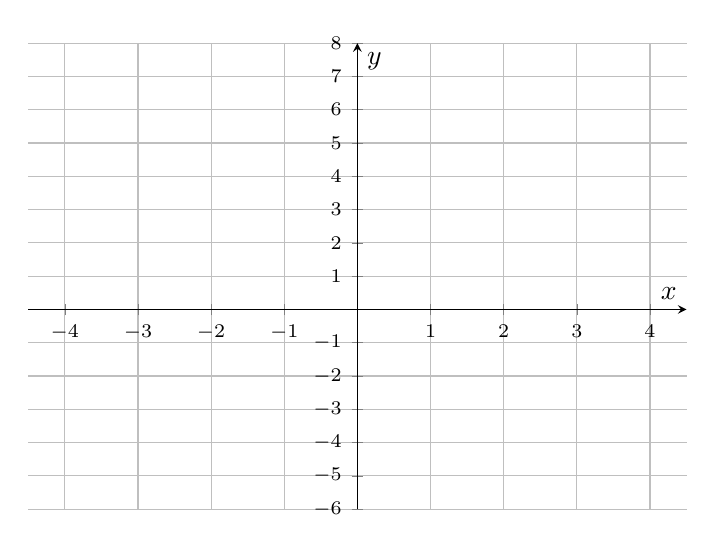
\begin{tikzpicture}
\begin{axis}[width=.82\linewidth,height=7.5cm,axis lines=middle,xmin=-4.5,xmax=4.5,ymin=-6,ymax=8,
  xtick={-4,...,4},ytick={-6,...,8},grid=major,xlabel={$x$},ylabel={$y$},tick label style={font=\scriptsize}]
\end{axis}
\end{tikzpicture}
\end{center}
\item Montrer que, pour tout réel $x$ non nul, $f(-x)=-f(x)$. Quelle symétrie de $\mathcal{C}_f$ cela traduit-il ? Indiquer, pour chaque courbe, les droites dont elle se rapproche (asymptotes).
\end{enumerate}
}{%
\begin{enumerate}
\item Le calcul de $\dfrac2x$ ou $\dfrac3x$ demande de diviser par $x$ ; la division par $0$ est impossible. L'ensemble de définition est $\R^{*}=]-\infty;0[\cup]0;+\infty[$.
\item
\begin{center}\small
\begin{tabular}{|c|*{10}{c|}}
\hline
$x$ & $-4$ & $-3$ & $-2$ & $-1$ & $-0{,}5$ & $0{,}5$ & $1$ & $2$ & $3$ & $4$\\
\hline
$f(x)$ & $0{,}5$ & $0{,}67$ & $1$ & $2$ & $4$ & $-4$ & $-2$ & $-1$ & $-0{,}67$ & $-0{,}5$\\
\hline
$g(x)$ & $0{,}25$ & $0$ & $-0{,}5$ & $-2$ & $-5$ & $7$ & $4$ & $2{,}5$ & $2$ & $1{,}75$\\
\hline
\end{tabular}
\end{center}
\item
\begin{center}
\begin{tikzpicture}
\begin{axis}[width=.82\linewidth,height=7.5cm,axis lines=middle,xmin=-4.5,xmax=4.5,ymin=-6,ymax=8,
  xtick={-4,...,4},ytick={-6,...,8},grid=major,xlabel={$x$},ylabel={$y$},tick label style={font=\scriptsize}]
\addplot[mxteacher,very thick,samples=100,domain=-4.5:-0.34]{-2/x};
\addplot[mxteacher,very thick,samples=100,domain=0.25:4.5]{-2/x};
\addplot[mxwarn,very thick,samples=100,domain=-4.5:-0.43]{1+3/x};
\addplot[mxwarn,very thick,samples=100,domain=0.43:4.5]{1+3/x};
\addplot[mxwarn,dashed] coordinates {(-4.5,1)(4.5,1)};
\node[mxteacher,anchor=west] at (axis cs:2.2,-1.8) {$\mathcal{C}_f$};
\node[mxwarn,anchor=west] at (axis cs:2.2,3.2) {$\mathcal{C}_g$};
\end{axis}
\end{tikzpicture}
\end{center}
\item $f(-x)=-\dfrac{2}{-x}=\dfrac2x=-f(x)$. Les points de coordonnées $(x;f(x))$ et $(-x;-f(x))$ sont symétriques par rapport à l'origine : $\mathcal{C}_f$ est symétrique par rapport à l'origine $O$. Asymptotes : pour $\mathcal{C}_f$, les droites d'équations $x=0$ et $y=0$ ; pour $\mathcal{C}_g$, les droites d'équations $x=0$ et $y=1$ (la courbe de $g$ est symétrique par rapport au point $(0;1)$, car $g(-x)+g(x)=2$).
\end{enumerate}
}{5}

\mxexdef{24}{Comportement aux bornes et asymptotes}{%
Soit $h$ la fonction définie sur $\R^{*}$ par $h(x)=-1+\dfrac{5}{x}$.
\begin{enumerate}
\item Calculer $h(x)$ pour $x\in\{-10\,000;-1\,000;-100;100;1\,000;10\,000\}$. Que peut-on conjecturer sur $h(x)$ lorsque $x$ devient très grand en valeur absolue ? Quelle droite asymptote en déduit-on ?
\item Calculer $h(x)$ pour $x\in\{-0{,}1;-0{,}01;-0{,}001;0{,}001;0{,}01;0{,}1\}$. Décrire le comportement de $h(x)$ lorsque $x$ se rapproche de $0$, par valeurs négatives puis par valeurs positives. Quelle droite asymptote en déduit-on ?
\item Calculer $h(-5)$, $h(-1)$, $h(1)$ et $h(5)$, puis tracer l'allure de la courbe de $h$ et ses asymptotes dans le repère ci-dessous.
\begin{center}
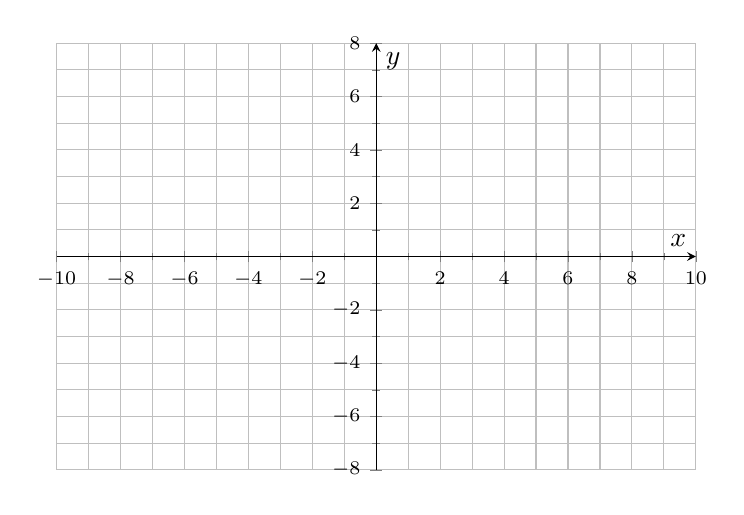
\begin{tikzpicture}
\begin{axis}[width=.8\linewidth,height=7cm,axis lines=middle,xmin=-10,xmax=10,ymin=-8,ymax=8,
  xtick={-10,-8,...,10},ytick={-8,-6,...,8},minor tick num=1,grid=both,xlabel={$x$},ylabel={$y$},tick label style={font=\scriptsize}]
\end{axis}
\end{tikzpicture}
\end{center}
\item Application. Un organisme de formation loue une salle $450$~€ la journée et dépense $12$~€ de repas par participant. Pour $x$ participants ($x\geqslant1$), le coût moyen par participant est $c(x)=12+\dfrac{450}{x}$ (en euros).
\begin{enumerate}[label=\alph*.]
\item Calculer $c(10)$, $c(50)$ et $c(150)$.
\item De quelle valeur le coût moyen se rapproche-t-il lorsque le nombre de participants devient très grand ? Peut-il devenir inférieur à $12$~€ ? Justifier.
\end{enumerate}
\end{enumerate}
}{%
\begin{enumerate}
\item $h(-10\,000)=-1{,}000\,5$ ; $h(-1\,000)=-1{,}005$ ; $h(-100)=-1{,}05$ ; $h(100)=-0{,}95$ ; $h(1\,000)=-0{,}995$ ; $h(10\,000)=-0{,}999\,5$. Quand $|x|$ devient très grand, $\dfrac5x$ se rapproche de $0$, donc $h(x)$ se rapproche de $-1$ (par valeurs inférieures en $-\infty$, supérieures en $+\infty$). La droite d'équation $y=-1$ est asymptote horizontale.
\item $h(-0{,}1)=-51$ ; $h(-0{,}01)=-501$ ; $h(-0{,}001)=-5\,001$ ; $h(0{,}001)=4\,999$ ; $h(0{,}01)=499$ ; $h(0{,}1)=49$. Quand $x$ se rapproche de $0$ par valeurs négatives, $h(x)$ devient négatif et aussi grand qu'on veut en valeur absolue ($h(x)\to-\infty$) ; par valeurs positives, $h(x)\to+\infty$. La droite d'équation $x=0$ est asymptote verticale.
\item $h(-5)=-2$, $h(-1)=-6$, $h(1)=4$, $h(5)=0$.
\begin{center}
\begin{tikzpicture}
\begin{axis}[width=.8\linewidth,height=7cm,axis lines=middle,xmin=-10,xmax=10,ymin=-8,ymax=8,
  xtick={-10,-8,...,10},ytick={-8,-6,...,8},minor tick num=1,grid=both,xlabel={$x$},ylabel={$y$},tick label style={font=\scriptsize}]
\addplot[mxteacher,very thick,samples=120,domain=-10:-0.72]{-1+5/x};
\addplot[mxteacher,very thick,samples=120,domain=0.56:10]{-1+5/x};
\addplot[mxwarn,dashed,thick] coordinates {(-10,-1)(10,-1)};
\addplot[only marks,mark=*,mxteacher] coordinates {(-5,-2)(-1,-6)(1,4)(5,0)};
\end{axis}
\end{tikzpicture}
\end{center}
\item
\begin{enumerate}[label=\alph*.]
\item $c(10)=12+45=57$~€ ; $c(50)=12+9=21$~€ ; $c(150)=12+3=15$~€.
\item Quand $x$ devient très grand, $\dfrac{450}{x}$ se rapproche de $0$ : le coût moyen se rapproche de $12$~€ (asymptote $y=12$). Comme $\dfrac{450}{x}>0$ pour $x>0$, on a toujours $c(x)>12$ : le coût moyen ne descend jamais sous $12$~€, le coût fixe de la salle se répartissant sur les participants sans disparaître.
\end{enumerate}
\end{enumerate}
}{5}

\mxexdef{25}{Dériver une somme polynôme et $k/x$}{%
Calculer la dérivée de chacune des fonctions suivantes, définies sur $\R^{*}$.
\begin{enumerate}[label=\alph*.]
\item $f(x)=5x+2-\dfrac{3}{x}$
\item $g(x)=-4x+7+\dfrac{6}{x}$
\item $h(x)=2x^3-5x^2+\dfrac{1}{x}$
\item $k(x)=\dfrac12x^2+4x-\dfrac{8}{x}$
\item $p(x)=\dfrac{x^2+2}{x}$ \quad (écrire d'abord $p(x)$ sous la forme $x+\dfrac{a}{x}$, puis donner $p'(x)$ sous la forme d'un seul quotient)
\end{enumerate}
}{%
On utilise : $(ax^n)'=nax^{n-1}$, la dérivée d'une constante est nulle et, pour $x\neq0$, $\left(\dfrac{k}{x}\right)'=k\times\left(-\dfrac1{x^2}\right)=-\dfrac{k}{x^2}$.
\begin{enumerate}[label=\alph*.]
\item $f'(x)=5-\left(-\dfrac{3}{x^2}\right)=5+\dfrac{3}{x^2}$.
\item $g'(x)=-4-\dfrac{6}{x^2}$.
\item $h'(x)=6x^2-10x-\dfrac{1}{x^2}$.
\item $k'(x)=x+4+\dfrac{8}{x^2}$.
\item $p(x)=\dfrac{x^2}{x}+\dfrac{2}{x}=x+\dfrac2x$, donc $p'(x)=1-\dfrac2{x^2}=\dfrac{x^2-2}{x^2}$.
\end{enumerate}
Erreur fréquente : écrire $\left(\dfrac{3}{x}\right)'=\dfrac{3}{x^2}$ en oubliant le signe « $-$ ».
}{5}

\mxexdef{26}{Dérivée factorisée, signe et variations}{%
Soit $f$ la fonction définie sur $\R^{*}$ par $f(x)=9x-2+\dfrac{4}{x}$.
\begin{enumerate}
\item Montrer que, pour tout réel $x$ non nul, $f'(x)=\dfrac{(3x-2)(3x+2)}{x^2}$.
\item Étudier le signe de $f'(x)$ sur $\R^{*}$ à l'aide d'un tableau de signes.
\item En déduire le tableau de variations de $f$, en y faisant figurer les valeurs de $f\!\left(-\dfrac23\right)$ et $f\!\left(\dfrac23\right)$.
\item Comparer $f\!\left(-\dfrac23\right)$ et $f\!\left(\dfrac23\right)$. Un maximum local peut-il être inférieur à un minimum local ? Expliquer à l'aide du tableau.
\end{enumerate}
}{%
\begin{enumerate}
\item $f'(x)=9-\dfrac{4}{x^2}=\dfrac{9x^2-4}{x^2}=\dfrac{(3x-2)(3x+2)}{x^2}$ (identité $a^2-b^2=(a-b)(a+b)$ avec $a=3x$, $b=2$).
\item $x^2>0$ pour $x\neq0$ : le signe de $f'(x)$ est celui de $(3x-2)(3x+2)$. $3x+2=0\iff x=-\dfrac23$ ; $3x-2=0\iff x=\dfrac23$.
\[
\begin{array}{|c|ccccccccc|}
\hline
x & -\infty & & -\frac23 & & 0 & & \frac23 & & +\infty\\ \hline
3x+2 & & - & 0 & + & \| & + & & + & \\
3x-2 & & - & & - & \| & - & 0 & + & \\
x^2 & & + & & + & 0 & + & & + & \\ \hline
f'(x) & & + & 0 & - & \| & - & 0 & + & \\ \hline
\end{array}
\]
\item $f\!\left(-\dfrac23\right)=-6-2-6=-14$ et $f\!\left(\dfrac23\right)=6-2+6=10$.
\[
\begin{array}{|c|ccccccccc|}
\hline
x & -\infty & & -\frac23 & & 0 & & \frac23 & & +\infty\\ \hline
f(x) & & \nearrow & -14 & \searrow & \| & \searrow & 10 & \nearrow & \\ \hline
\end{array}
\]
$f$ est croissante sur $\left]-\infty;-\dfrac23\right]$, décroissante sur $\left[-\dfrac23;0\right[$ et sur $\left]0;\dfrac23\right]$, croissante sur $\left[\dfrac23;+\infty\right[$.
\item $-14<10$ : le maximum local (atteint en $-\dfrac23$, sur $]-\infty;0[$) est inférieur au minimum local (atteint en $\dfrac23$, sur $]0;+\infty[$). Ce n'est pas contradictoire : ce sont des extremums locaux sur deux intervalles séparés par la valeur interdite $0$, où la courbe « saute » (asymptote verticale).
\end{enumerate}
}{4}

\mxexdef{27}{Dérivée toujours positive et signe d'un quotient}{%
Soit $h$ la fonction définie sur $\R^{*}$ par $h(x)=2x-3-\dfrac{5}{x}$.
\begin{enumerate}
\item Montrer que, pour tout réel $x$ non nul, $h'(x)=\dfrac{2x^2+5}{x^2}$.
\item Étudier le signe de $h'(x)$ et en déduire les variations de $h$.
\item Calculer $h(-1)$ et $h(1)$. Peut-on dire que « $h$ est croissante sur $\R^{*}$ » ? Expliquer.
\item Montrer que, pour tout réel $x$ non nul, $h(x)=\dfrac{(2x-5)(x+1)}{x}$. Dresser le tableau de signes de $h(x)$, puis résoudre l'inéquation $h(x)\geqslant0$.
\end{enumerate}
}{%
\begin{enumerate}
\item $h'(x)=2-\left(-\dfrac{5}{x^2}\right)=2+\dfrac{5}{x^2}=\dfrac{2x^2+5}{x^2}$.
\item Pour $x\neq0$ : $2x^2+5\geqslant5>0$ et $x^2>0$, donc $h'(x)>0$. La fonction $h$ est strictement croissante sur $]-\infty;0[$ et strictement croissante sur $]0;+\infty[$.
\[
\begin{array}{|c|ccccc|}
\hline
x & -\infty & & 0 & & +\infty\\ \hline
h'(x) & & + & \| & + & \\ \hline
h(x) & & \nearrow & \| & \nearrow & \\ \hline
\end{array}
\]
\item $h(-1)=-2-3+5=0$ et $h(1)=2-3-5=-6$. On a $-1<1$ mais $h(-1)>h(1)$ : $h$ n'est pas croissante sur $\R^{*}$ tout entier. Elle est croissante sur chacun des deux intervalles, séparément.
\item $\dfrac{(2x-5)(x+1)}{x}=\dfrac{2x^2-3x-5}{x}=2x-3-\dfrac5x=h(x)$. Valeurs critiques : $-1$, $0$ (valeur interdite) et $\dfrac52$.
\[
\begin{array}{|c|ccccccccc|}
\hline
x & -\infty & & -1 & & 0 & & \frac52 & & +\infty\\ \hline
2x-5 & & - & & - & & - & 0 & + & \\
x+1 & & - & 0 & + & & + & & + & \\
x & & - & & - & 0 & + & & + & \\ \hline
h(x) & & - & 0 & + & \| & - & 0 & + & \\ \hline
\end{array}
\]
L'ensemble des solutions de $h(x)\geqslant0$ est $[-1;0[\cup\left[\dfrac52;+\infty\right[$ ($0$ est exclu car valeur interdite). Contrôle : $h(-0{,}5)=6>0$, $h(1)=-6<0$, $h(3)=\dfrac43>0$.
\end{enumerate}
}{5}

\mxexdef{28}{Dérivée et variations de la fonction inverse}{%
Soit $f$ la fonction inverse, définie sur $\R^{*}$ par $f(x)=\dfrac1x$.
\begin{enumerate}
\item Soit $h$ un réel non nul, avec $h\neq-2$. Montrer que le taux de variation de $f$ entre $2$ et $2+h$ vaut
$\dfrac{f(2+h)-f(2)}{h}=-\dfrac{1}{2(2+h)}$. En faisant tendre $h$ vers $0$, en déduire $f'(2)$.
\item On admet que, pour tout réel $x$ non nul, $f'(x)=-\dfrac1{x^2}$. Vérifier la cohérence avec la question 1, puis calculer $f'(-1)$ et $f'(0{,}5)$.
\item Étudier le signe de $f'(x)$ et dresser le tableau de variations de $f$.
\item Un élève remarque que $-2<3$ et $f(-2)<f(3)$, et affirme que cela contredit la décroissance de $f$. Que lui répondre ?
\end{enumerate}
}{%
\begin{enumerate}
\item $f(2+h)-f(2)=\dfrac1{2+h}-\dfrac12=\dfrac{2-(2+h)}{2(2+h)}=\dfrac{-h}{2(2+h)}$. En divisant par $h\neq0$ : $\dfrac{f(2+h)-f(2)}{h}=-\dfrac1{2(2+h)}$. Lorsque $h$ tend vers $0$, ce taux tend vers $-\dfrac1{2\times2}=-\dfrac14$ : $f'(2)=-\dfrac14$.
\item $-\dfrac1{2^2}=-\dfrac14$ : cohérent. $f'(-1)=-\dfrac1{(-1)^2}=-1$ et $f'(0{,}5)=-\dfrac1{0{,}25}=-4$ (pentes des tangentes en ces points).
\item Pour $x\neq0$, $x^2>0$, donc $f'(x)=-\dfrac1{x^2}<0$.
\[
\begin{array}{|c|ccccc|}
\hline
x & -\infty & & 0 & & +\infty\\ \hline
f'(x) & & - & \| & - & \\ \hline
f(x) & & \searrow & \| & \searrow & \\ \hline
\end{array}
\]
$f$ est strictement décroissante sur $]-\infty;0[$ et strictement décroissante sur $]0;+\infty[$.
\item $f(-2)=-0{,}5$ et $f(3)\approx0{,}33$ : on a bien $f(-2)<f(3)$. Il n'y a pas de contradiction : $-2$ et $3$ ne sont pas dans le même intervalle. La fonction inverse est décroissante sur chaque intervalle séparément, pas sur $\R^{*}$ tout entier ; on ne peut comparer des images avec le sens de variation que pour deux réels d'un même intervalle.
\end{enumerate}
}{4}

\mxexdef{29}{Lecture graphique d'un coût moyen}{%
Une entreprise assemble entre $10$ et $70$ vélos électriques par mois. Pour $x$ vélos assemblés, on note $C(x)$ le coût de production unitaire moyen, en euros. La courbe de la fonction $C$ sur $[10;70]$ est donnée ci-dessous.
\begin{center}
\begin{tikzpicture}
\begin{axis}[width=.85\linewidth,height=7.5cm,xmin=10,xmax=70,ymin=650,ymax=1050,
  xtick={10,15,...,70},ytick={650,700,...,1050},minor y tick num=1,grid=both,
  xlabel={nombre de vélos $x$},ylabel={$C(x)$ en €},tick label style={font=\scriptsize},label style={font=\small}]
\addplot[mxteacher,very thick,samples=150,domain=10:70]{8*x+200+7200/x};
\end{axis}
\end{tikzpicture}
\end{center}
\begin{enumerate}
\item Lire le coût unitaire moyen lorsque l'entreprise assemble $15$ vélos, puis $50$ vélos.
\item Pour quelles productions le coût unitaire moyen est-il égal à $800$~€ ?
\item Quel est le coût unitaire moyen minimal ? Pour quelle production est-il atteint ?
\item On admet que $C(x)=8x+200+\dfrac{7\,200}{x}$. Calculer $C'(x)$, vérifier que $C'(x)=\dfrac{8(x-30)(x+30)}{x^2}$ et confirmer par le calcul la réponse à la question 3.
\end{enumerate}
}{%
Exiger des traits de lecture (pointillés) et des unités ; une lecture graphique est approchée.
\begin{enumerate}
\item On lit $C(15)\approx800$~€ et $C(50)\approx745$~€ (valeur exacte avec la formule de la question 4 : $744$~€).
\item On trace la droite d'équation $y=800$ : elle coupe la courbe aux points d'abscisses $15$ et $60$. Le coût moyen vaut $800$~€ pour $15$ ou $60$ vélos.
\item Le point le plus bas de la courbe a pour coordonnées environ $(30;680)$ : coût minimal d'environ $680$~€ par vélo, pour $30$ vélos par mois.
\item $C'(x)=8-\dfrac{7\,200}{x^2}=\dfrac{8x^2-7\,200}{x^2}=\dfrac{8(x^2-900)}{x^2}=\dfrac{8(x-30)(x+30)}{x^2}$. Sur $[10;70]$, $x+30>0$ et $x^2>0$ : $C'(x)$ a le signe de $x-30$, négatif sur $[10;30[$ et positif sur $]30;70]$. $C$ est décroissante sur $[10;30]$ puis croissante sur $[30;70]$ ; son minimum est $C(30)=240+200+240=680$~€. Contrôles : $C(15)=120+200+480=800$ et $C(60)=480+200+120=800$.
\end{enumerate}
}{5}

\mxexdef{30}{Minimiser un coût moyen par la dérivée}{%
Une plateforme de compostage produit chaque semaine $x$ tonnes de compost, avec $x\in[2;25]$. Le coût total hebdomadaire de production, en euros, est modélisé par $C(x)=2x^2+40x+288$.
On note $f$ la fonction qui donne le coût moyen de production d'une tonne : $f(x)=\dfrac{C(x)}{x}$.
\begin{enumerate}
\item Montrer que, pour tout $x\in[2;25]$, $f(x)=2x+40+\dfrac{288}{x}$.
\item Calculer $f'(x)$ et montrer que, pour tout $x\in[2;25]$, $f'(x)=\dfrac{2(x-12)(x+12)}{x^2}$.
\item Étudier le signe de $f'(x)$ sur $[2;25]$ et dresser le tableau de variations de $f$ (valeurs aux bornes comprises).
\item Quel est le coût moyen minimal d'une tonne de compost ? Pour quelle production hebdomadaire est-il atteint ? Quel est alors le coût total de la semaine ?
\end{enumerate}
}{%
\begin{enumerate}
\item Pour $x\in[2;25]$, $x\neq0$ : $f(x)=\dfrac{2x^2}{x}+\dfrac{40x}{x}+\dfrac{288}{x}=2x+40+\dfrac{288}{x}$.
\item $f'(x)=2-\dfrac{288}{x^2}=\dfrac{2x^2-288}{x^2}=\dfrac{2(x^2-144)}{x^2}=\dfrac{2(x-12)(x+12)}{x^2}$.
\item Sur $[2;25]$ : $2>0$, $x+12>0$ et $x^2>0$, donc $f'(x)$ a le signe de $x-12$ : $f'(x)<0$ sur $[2;12[$, $f'(12)=0$, $f'(x)>0$ sur $]12;25]$.
$f(2)=4+40+144=188$ ; $f(12)=24+40+24=88$ ; $f(25)=50+40+11{,}52=101{,}52$.
\[
\begin{array}{|c|ccccc|}
\hline
x & 2 & & 12 & & 25\\ \hline
f'(x) & & - & 0 & + & \\ \hline
f(x) & 188 & \searrow & 88 & \nearrow & 101{,}52\\ \hline
\end{array}
\]
\item Le coût moyen minimal est de $88$~€ par tonne, atteint pour une production de $12$ tonnes par semaine. Le coût total est alors $C(12)=288+480+288=1\,056$~€ (contrôle : $12\times88=1\,056$).
\end{enumerate}
}{4}
